
\subsection{Experimental Setup}
\label{sec:experimental_setup}
To evaluate the proposed models and job scheduling policies, we have access to 128 nodes
of the Quartz cluster, as described in Section \ref{sec:platforms}.  We use an in-house
simulator to mimic the behavior of a job scheduling system on a production platform like
Quartz.  The simulator is described in more detail in Section \ref{sec:simulator}. 
For training the prediction models, we use the set of kernel and micro-benchmark
applications described in Section~\ref{sec:benchmarks}.  Our benchmark applications used 
as the cluster's workload are also described in Section \ref{sec:benchmarks}.  They
consist of a mix of single and multi-node applications.  Single node ones can run on a
single node, while multi-node ones require a number of sockets.  We append the number of
processes used at the end of the name of each multi-node application.  They range from 8
to 64 processes and each process is scheduled on a single socket.  For example, an 8 process
application requires 8 sockets (4 nodes) to run.  We maintain socket temperature
between 38-42 $^\circ$C, in order to only observe the power consumption variation relevant
to manufacturing variability.  Based on the data and independent nature of jobs run on HPC
clusters, we expect the observed trends in this work to scale on larger systems. 

\begin{figure}[t!]
	\centering
	\begin{subfigure}[b]{.9\columnwidth}
		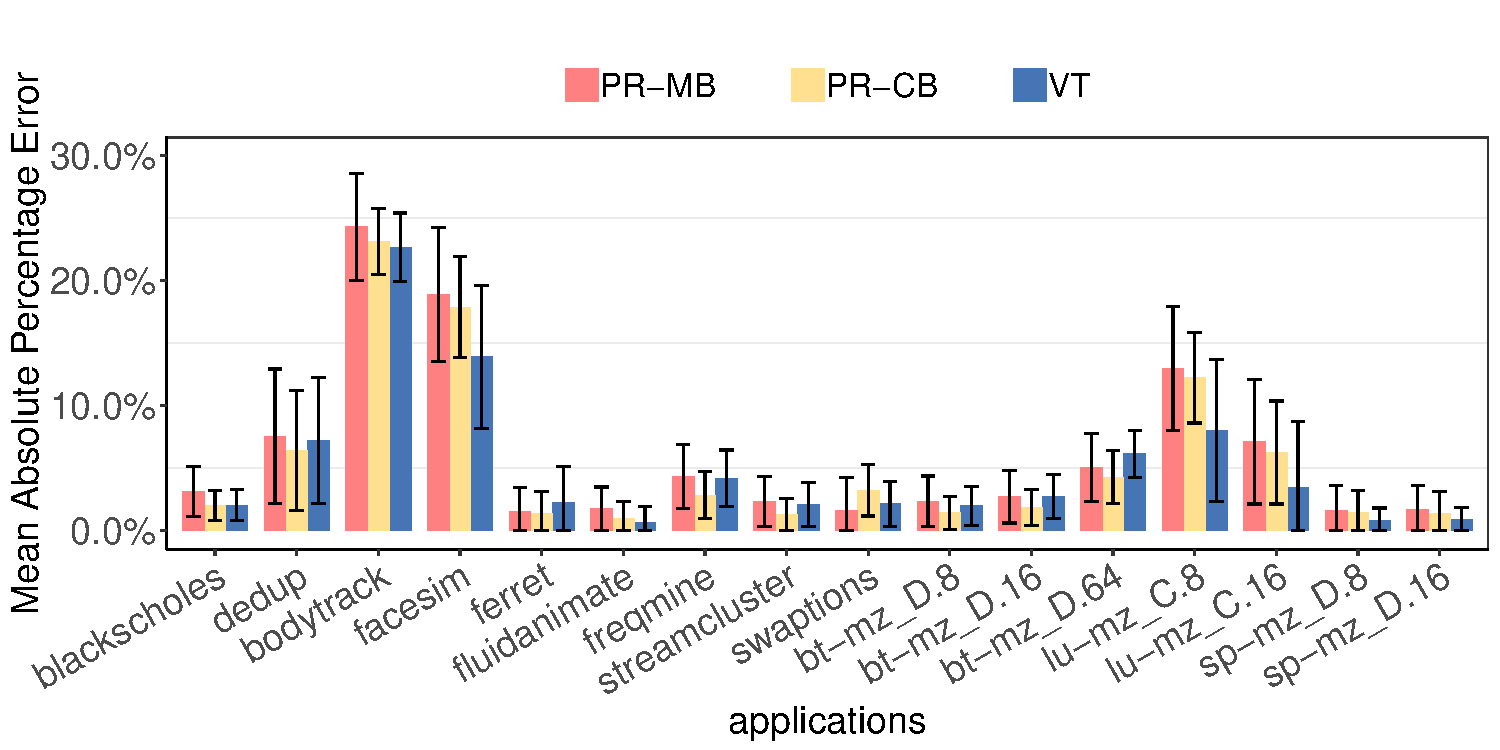
\includegraphics[width=\textwidth]{power_aware_job_scheduling/figures/model_power_pred_error}
	\end{subfigure}%
	\caption{Comparison of average power prediction error for all models over all sockets.
The error bars show the standard error deviation across all sockets for the corresponding
application.}
	\label{fig:model_power_pred_error}
\end{figure}

\subsection{Model Validation}
\label{sec:model_validation}

In this section we experimentally validate the prediction models presented in
Section~\ref{sec:variability_prediction}.  We analyze the models in terms of Mean Absolute
Percentage Error (MAPE) (see Equation \ref{eq:mape})  between predicted and real values.
Figure~\ref{fig:model_power_pred_error} shows the MAPE values of the average power
predictions for all applications over all sockets.  The error bars show the standard
deviation of the MAPE metric, computed over all the 256 sockets.  These results correspond
to the optimized versions of the Power Ratio (PR) prediction model, presented in
Section~\ref{sec:naive_model}, and the Variability-Trained (VT), which is presented in
Section~\ref{sec:pmcs_model}.  Since the PR model incorrectly assumes that all
applications are affected by manufacturing variability the same way, we show two versions
of the PR. Models are denoted as PR-MB and PR-CB, using by a memory bound
(\textit{sparseLU}) and a computation bound benchmark (\textit{cholesky}) for computing
the variability ratios, respectively.  Overall, all models performs well, achieving an
average error below 10\%.  The VT model outperforms the PR models, while PR models varies
depending on the benchmark used to compute the variability ratios.  PR-MB consistently
performs worse than PR-CB, since the memory bound benchmark detects up to 15\% less
variability than the computation bound one.  This disparity among results for the PR model
can become a more serious problem in the future, as variability is expected to increase
\cite{Marathe:2017:ESP:3149412.3149421}.  The more robust VT model will be better suited,
since it does not falsely assume that variability is application independent.  The
unoptimized versions (see Section \ref{sec:variability_prediction}) of the same models
perform again similarly among themselves, but significantly worse that their optimized
counterparts shown in figure \ref{fig:model_power_pred_error}.  On average, all
unoptimized model versions' error reach up to 16\% (results not shown).
\par
Our results show that all three models are able to predict the power consumption
variability in some cases.  However, it is possible to miss-predict if an application's
behavior is not well represented by the benchmarks used for training.Two such cases
are \textit{bodytrack} and \textit{facesim},  that although they are effectively using more
than 8 cores, their power consumption remains below 60 Watts.  Moreover, PR-MB and PR-CB
additionally fail to produce accurate predictions for \textit{lu-mz\_C.8}, which use only
a single core on each socket.  Higher prediction errors can impact the effectiveness of
the scheduling policies that rely on them, causing them to over-estimate a job's power
consumption.  Over-estimating power can lead to underutilization of the cluster's
resources.  Even high error values though, such as in the case of \textit{bodytrack}, are
better and more robust approximations of the actual power consumption than user
estimations, which comes with no guarantees. 

\subsection{Variability-Aware Scheduling Evaluation}
\label{sec:var_sched_eval}

In this Section we evaluate the two novel scheduling policies, \PRVSSched~ and
\PMCVSSched~, which are presented in Section~\ref{sec:job_sched_scheduling}.  We compare them to
four other scheduling policies, \DefaultSched~, \PESched~, \PEVASched~ and \IVSSched~,
which are also described in~\ref{sec:job_sched_scheduling}.  \DefaultSched~ policy implements
SLURM's logic in our simulator, with the addition of power-awareness and power
backfilling.  \PESched~ and \PEVASched~ employ state-of-the-art features of power-aware
policies ~\cite{patki:2013:eho:2464996.2465009,7515666,Gholkar:2016:PTH:2967938.2967961},
while \IVSSched~ demonstrates the ideal scenario, where prediction is 100\% accurate.  In
the case of \PRVSSched~ we use \textit{cholesky} to produce the variability ratios
required by the PR model, since it produces more accurate predictions than
\textit{sparseLU} (see Section \ref{sec:model_validation}).  The evaluation is done based
on a simulator, as described in Section~\ref{sec:experimental_setup}, by feeding it
performance and power traces from actual executions on the Quartz cluster.  For our
experiments we generate random job workloads composed of nine applications from the
PARSECSs suite and seven multi-node jobs from NAS-MZ, simulating both bursty and heavy
traffic scenarios (see Section~\ref{sec:experimental_setup}).  The main objective of each
policy is to improve the cluster's performance and energy consumption, while keeping the
total energy consumption below a certain global power budget.  All policies treat power as
a limited resource and depending on a predicted or estimated power peak for each job, they
restrict the number of running jobs to only those that can be accommodated by the given
global power budget.  

\begin{figure*}[ht]
	\centering
  \begin{subfigure}[b]{\textwidth}
    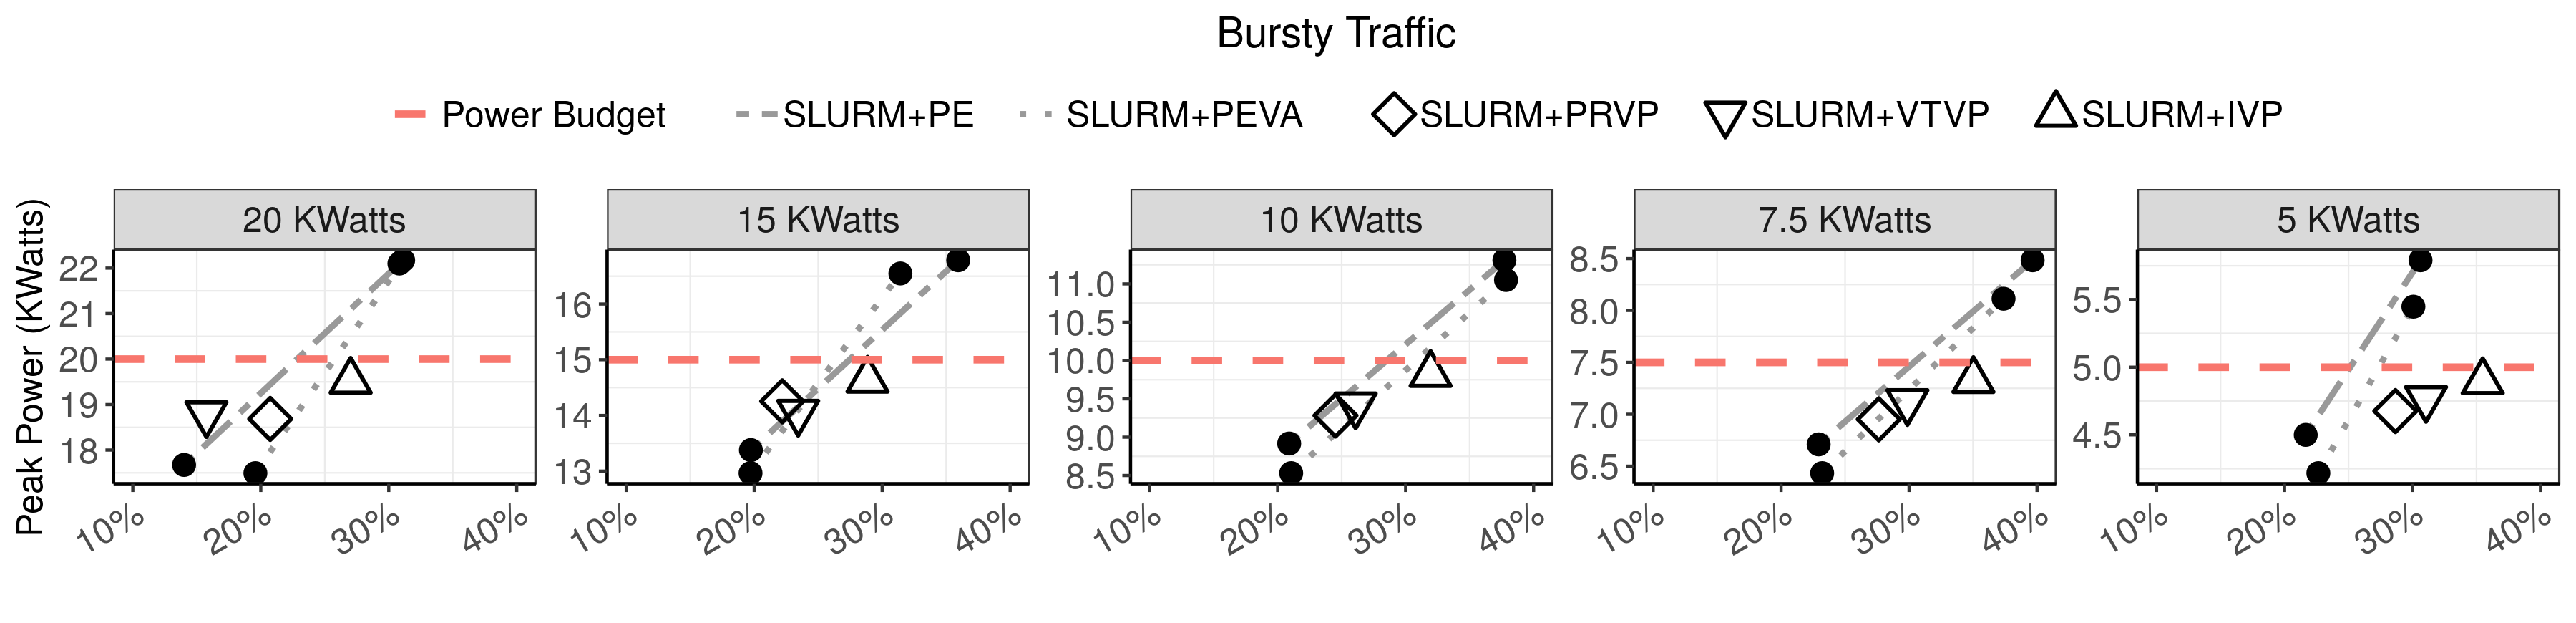
\includegraphics[width=\textwidth]{power_aware_job_scheduling/figures/peakPower2avgTurnaroundTime_bursty}
  \end{subfigure}%
	\qquad
 	\vspace{-.5cm} 
	\begin{subfigure}[b]{\textwidth}
    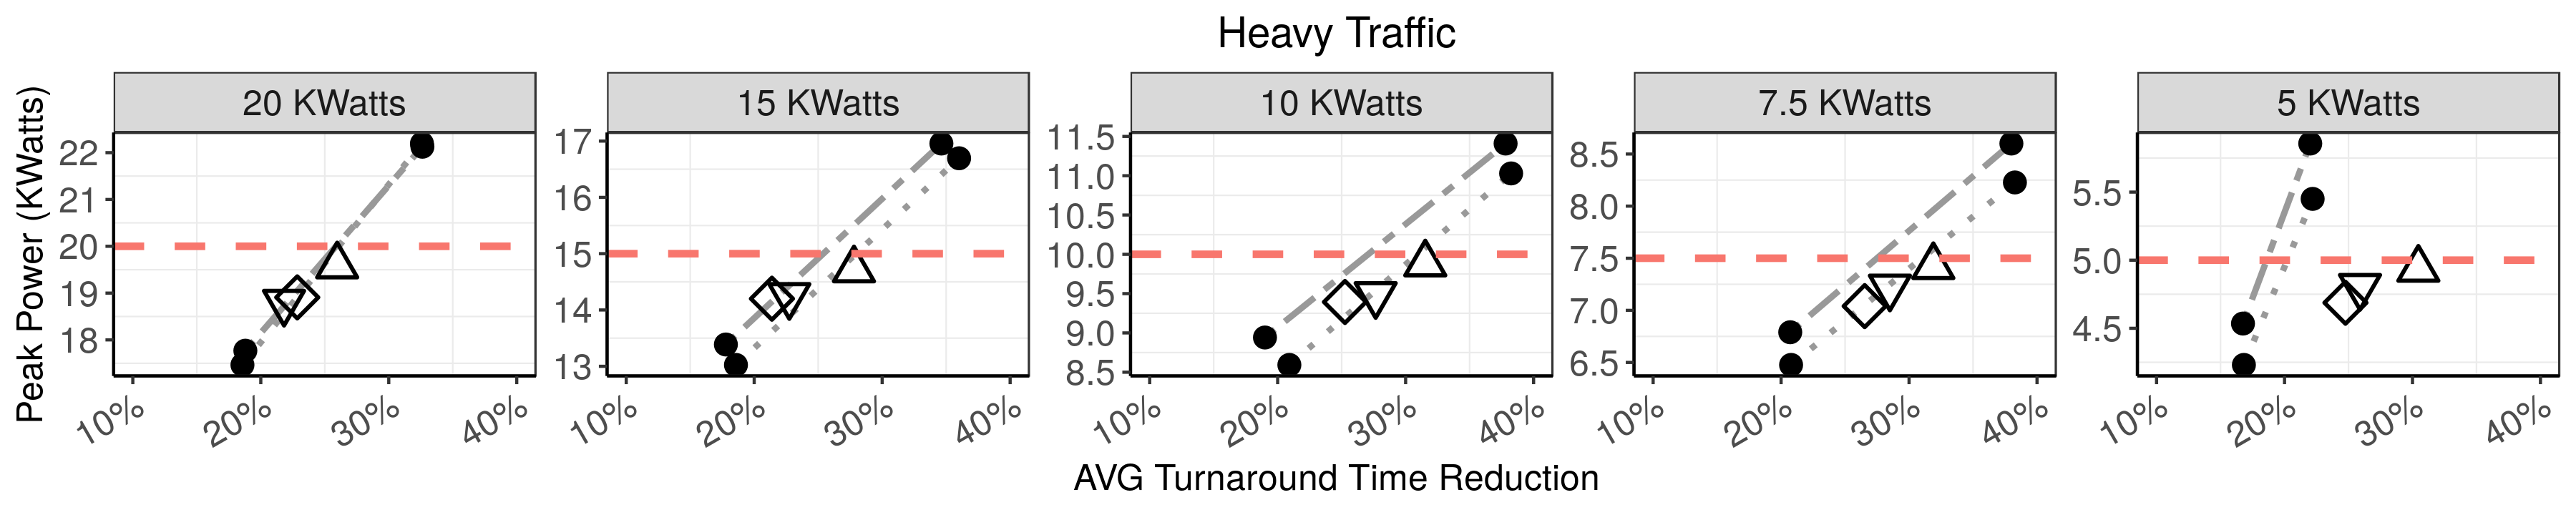
\includegraphics[width=\textwidth]{power_aware_job_scheduling/figures/peakPower2avgTurnaroundTime_heavy}
  \end{subfigure}%
 	\vspace{.3cm} 
	\caption{Power and Average turnaround time reduction over SLURM extended.  Results 
					SLURM+PE and SLURM+PEVA values range as shown by the corresponding lines, 
					depending on the estimation provided.}
	\label{fig:avg_turnaround_time}
\end{figure*}



\par
Figure~\ref{fig:avg_turnaround_time} compares the different policies in terms of average
job turnaround time reduction (x axis) and their maximum power consumption (y axis).  The
turnaround time reduction shown in percentages on x axis is over the \DefaultSched~
policy, for the corresponding power budget and traffic.  We define job turnaround time as
the time a job waits to be scheduled, including scheduler overhead, plus its execution
time.  The average job turnaround time is computed as the sum of turnaround time of all
jobs, divided by the number these jobs.  Results consider four different system-wide power
budgets, 5K, 7.5K, 10K, 15K and 20KWatts and the bursty and heavy traffic scenarios
described in Section~\ref{sec:experimental_setup}.  Our workloads require 25K Watts to run
using the whole cluster without any power restrictions.  In the 5KW case, the
\DefaultSched~ is forced to drop jobs that use 64 sockets, since it estimates that these
jobs require more power than available to the system.  The minimum budget that allows
\DefaultSched~ to run jobs that demand 64 sockets is 7.5KW.  Since the case of 5KW
\DefaultSched~ runs a lighter load (dropped 64 socket jobs), results are slightly biased
towards \DefaultSched~ (just for the 5KW case).

\begin{figure}[ht!]
	\centering
  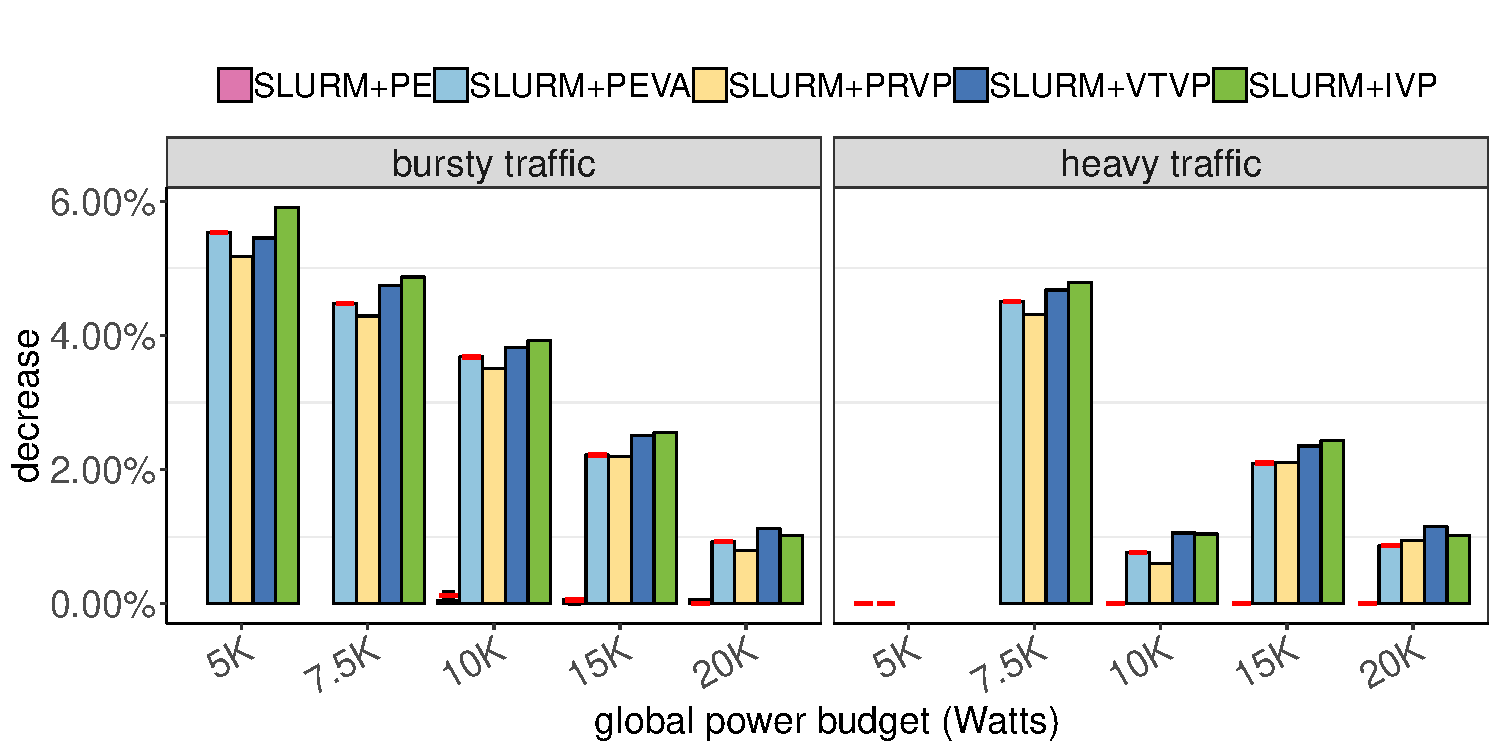
\includegraphics[width=.9\columnwidth]{power_aware_job_scheduling/figures/total_energy_115W}
	\caption{Energy consumption Reduction over \DefaultSched, under different budgets and 
					traffic scenarios. SLURM+PE, which is variability agnostic fail to save any energy,
					while SLURM+VTVP performs best.}
	\label{fig:total_energy_consumption}
%	\vspace{-.3cm}
\end{figure}

\par
\PRVSSched, \PMCVSSched~ and \IVSSched~ policies are denoted with different symbols.  The
two considered traffic scenarios produce similar results.  Except for the budget of
20KWatts, \PMCVSSched~ performs marginally better (up to 2\%) than \PRVSSched, which
reflects the better precision of its model.  The lowest reduction in terms of job
turnaround time, \EstMaxJTT\%, is observed in the case of the bursty traffic scenario,
under a power budget of 20KWatts, for the \PMCVSSched~ policy.  The largest improvement,
\EstMinJTT\%, is obtained by the \PMCVSSched~ policy when managing the bursty traffic
under a power budget of 5KWatts.  The benefits of the \PRVSSched, and the \PMCVSSched~
policies reach an average of \AvgJTT\%, considering all power budgets and traffic
scenarios.  \IVSSched, which is the ideal scenario, performs slightly better than
\PRVSSched and \PMCVSSched under all power budgets, although the benefits achieved by our
two proposed policies are very close to the best possible scheduling.  \PESched~ and
\PEVASched~ are shown as lines, where their performance and maximum power consumption can
lie on any point on the corresponding line.  This is because unlike our proposed policies,
which use prediction models to compute the power consumption of each job on each socket,
the power-estimation-based policies, \PESched~ and \PEVASched, use a single power
estimation obtained from power profiling on a single socket.  Due to the power variability
of each socket, it is possible that the estimation varies according to the variability of
the socket used for profiling.  This variance impacts the policies' efficiency.
Underestimating power by using a power efficient socket allows more sockets to get
allocated, but the net power consumption of the system can exceed the system-wide power
budget.  Contrary, overestimating power can lead to significant performance degradation,
since the policy becomes more conservative, underutilizing the available power budget.
Using a socket with moderate power consumption to get the power trace used for the
estimation can achieve comparable results to \PRVSSched, \PMCVSSched.  However, all points
on the lines showing the range of possible results for \PESched~ and \PEVASched~ show
worse reduction than \PRVSSched, \PMCVSSched~ and \IVSSched, since variability is not
considered.
%\par
%Considering power variability during scheduling decisions does not seem to play a major
%role here, since the variability-agnostic \PESched~ match the performance of the
%\PEVASched~ and potentially even the \PRVSSched~ and \PMCVSSched~ policies.  However, the
%accuracy of the estimation or prediction is important for improving turnaround time.
\par
Figure~\ref{fig:total_energy_consumption} shows the reduction in the system-wide energy
consumption. Both traffic scenarios' benefits increase as the system wide power budget is
reduced.  When less power is available, considering variability is important for energy
saving, since we can choose to always use the most power efficient sockets.  Note that
under heavy traffic, the 5K scenario offers no benefit.  This is because a significant
number of multi-node jobs are dropped by the \DefaultSched~ since they appear to require
more power than available to the system.  As a result, \DefaultSched~ runs a lighter
workload than he rest of the policies.  This also happens in the bursty scenario, but
since the workload only contains a few 64 socket jobs that are dropped, we still observe
significant benefits.  \PESched, which is variability-agnostic, offers no benefit over the
\DefaultSched~ policy.  \PEVASched, which prioritizes allocation of power efficient
sockets, matches the energy savings of the \PRVSSched~ and \PMCVSSched~ policies.
Accounting for power variability can have a significant impact on energy efficiency
reaching \MaxEnergy\% on the most energy-restricted scenarios.
\par
Results shown across Section~\ref{sec:job_scheduling_results} prove that our proposed
\PRVSSched~ and \PMCVSSched~\\
policies can improve energy efficiency up to \MaxEnergy\% (\AvgEnergy\% on
average) over simple solutions commonly used.  Moreover, job turnaround time is reduced up
to \MaxJTT\% (\AvgJTT\% on average).  Compared to the \PEVASched~ policy, which is
variability-aware, our method is more robust  as none of the  \PESched~ and \PEVASched~
policies can guarantee that the system-wide power budgets are respected. 

